\chapter{Requirements Capture}
%ability independently to formulate and solve technical problems in project work. 
%The project specification should state clearly what the project is intended to deliver, including all hardware, software, simulation.

\section{The Project Deliverable}
The objective of this project is to solve of problem of putting shoe laces on a shoe using bi-manual robot YuMi. Starting with one arm holding the shoelace, YuMi should detect a shoe hole and pass the shoelace through it by planning an arm trajectory. For more challenging version, YuMi will also plan sequences of trajectories to complete more holes up to the whole shoe.

\begin{figure}[H]
\centering
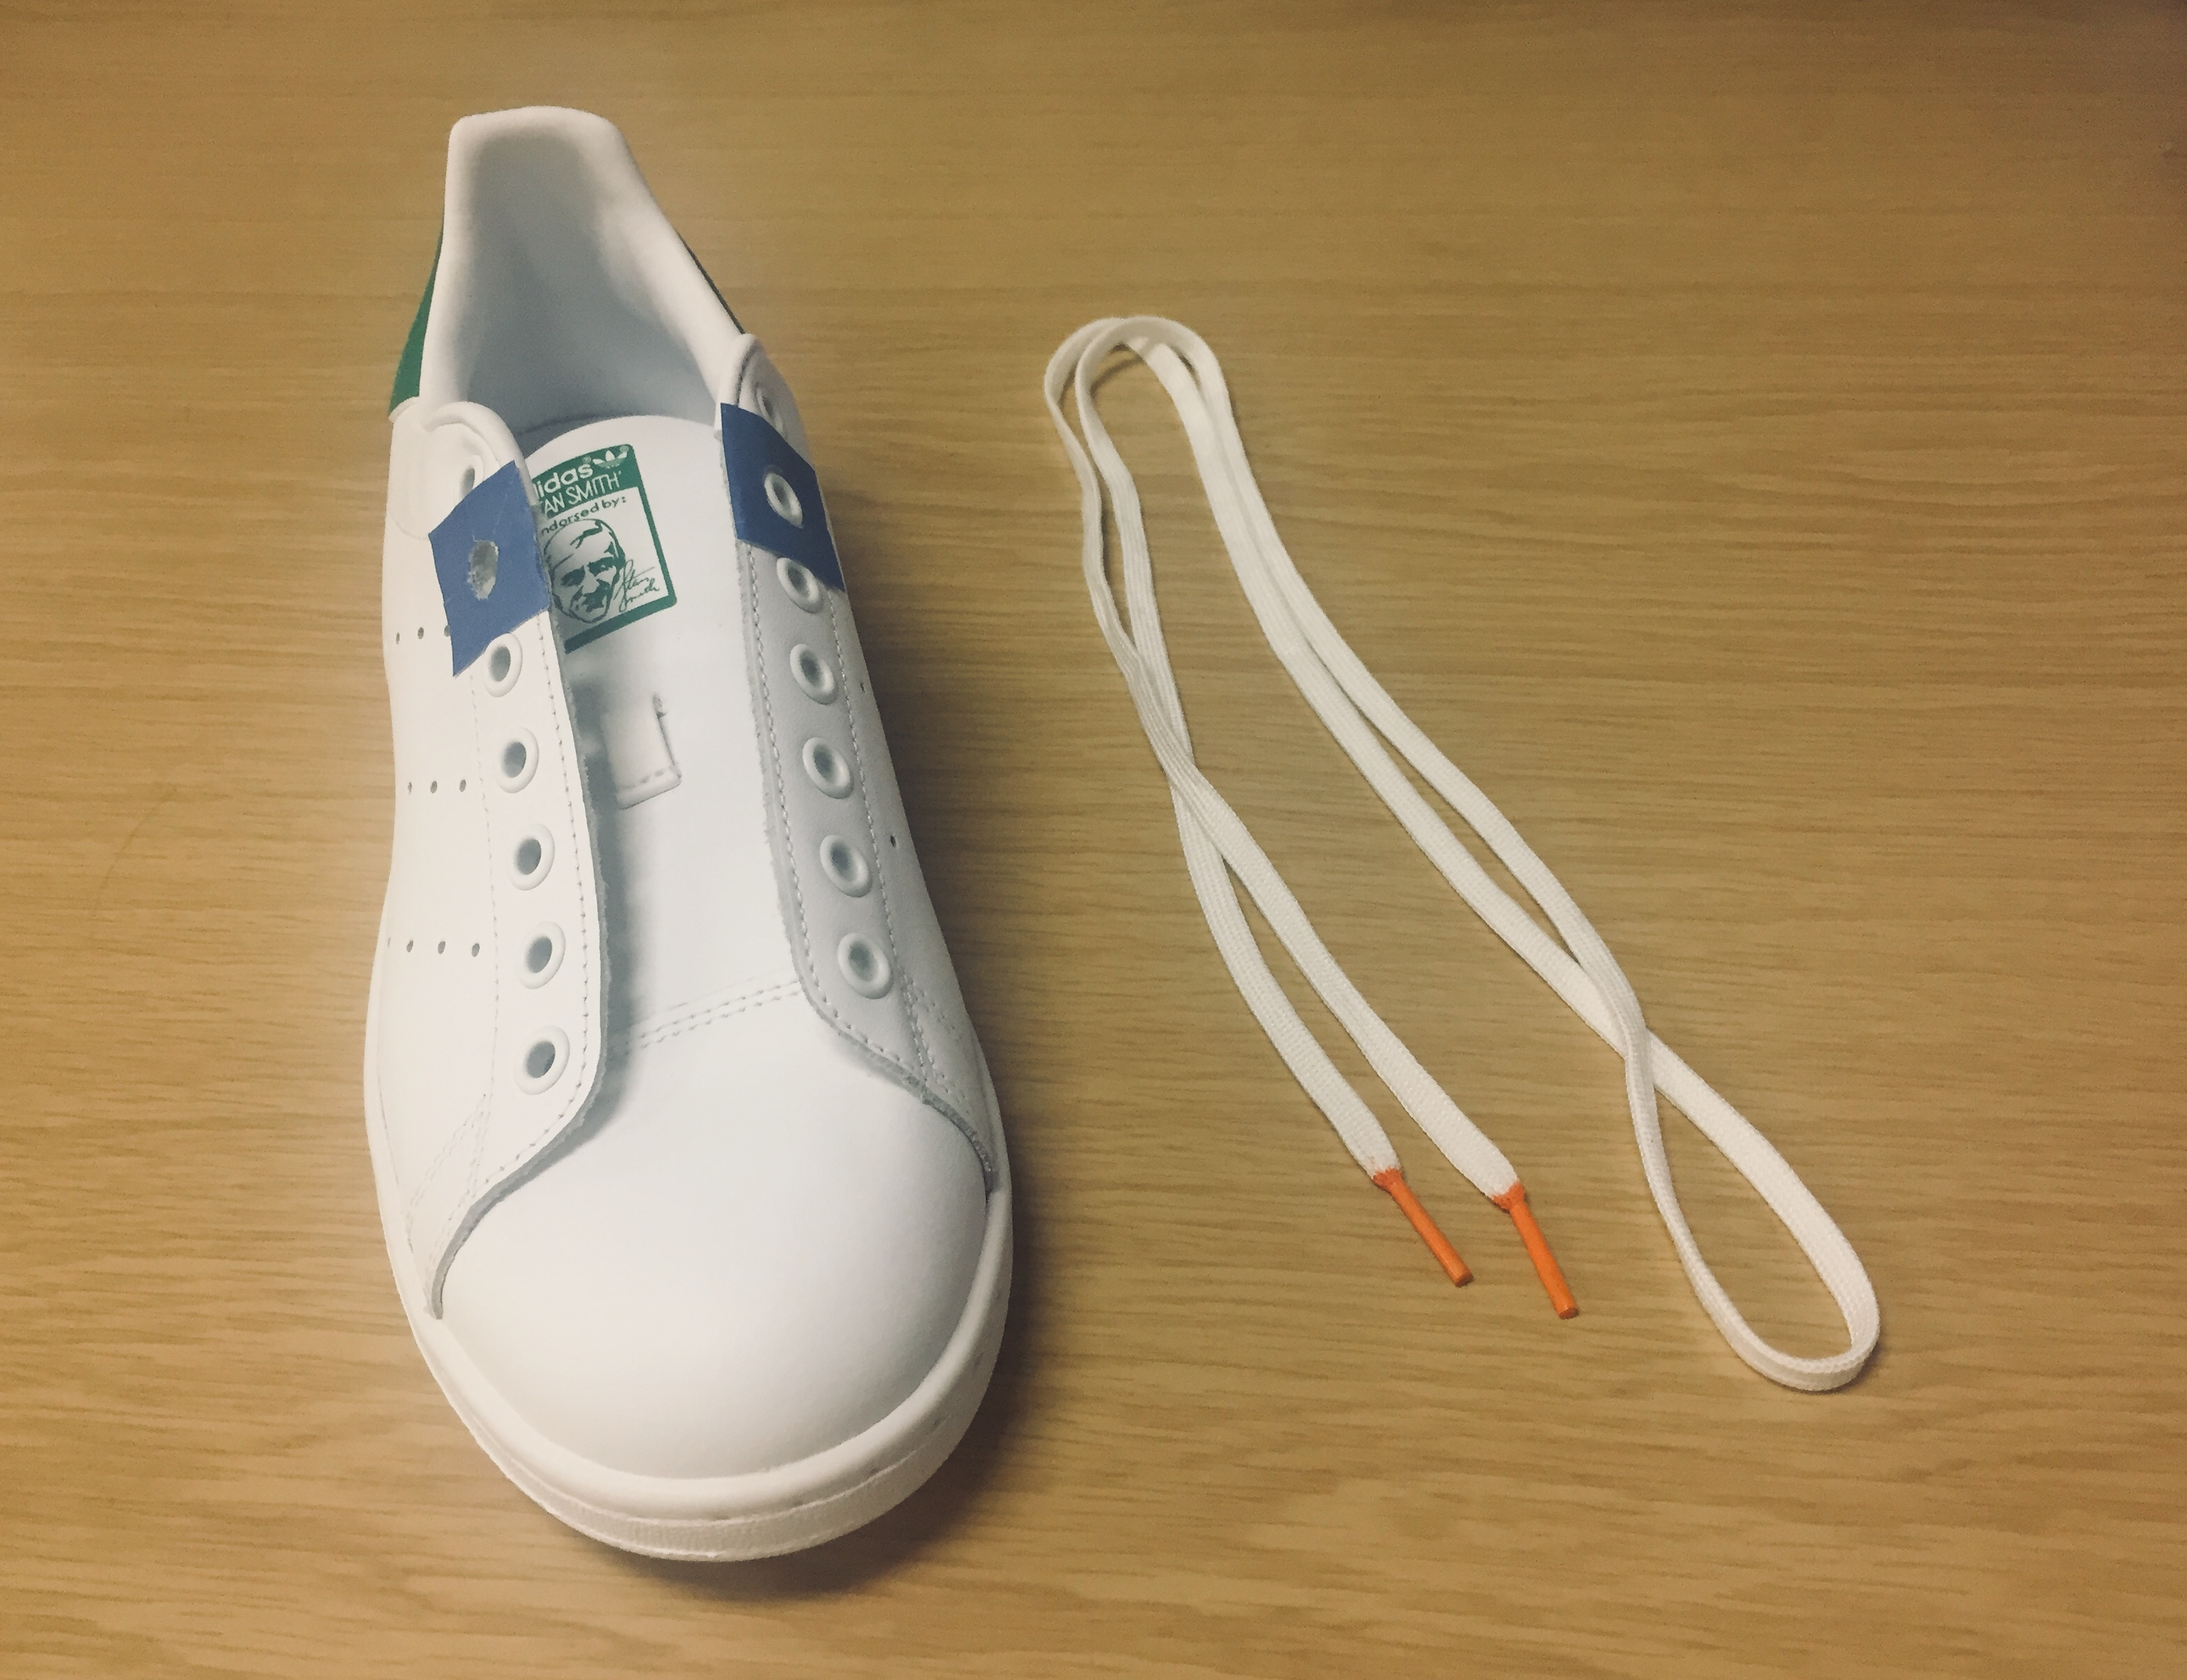
\includegraphics[width = 0.5\columnwidth]{RequirementsCap/shoe.jpg}
\caption{The manipulated shoe with distinct lace and hole colors}
\label{shoe}
\end{figure}

To constrain the problem, a shoe with distinct lace and hole colors will be used as the target for manipulation, which is shown in Figure \ref{shoe}. In addition, the entire manipulation process will be carried out on the workbench of the Imperial College Personal Robotics Lab under normal lighting condition.

The project deliverables can be divided into two main parts: Computer Vision and Motion Planning.

\section{Computer Vision}
The main aim of this part is to compute the real-time 6D pose of a specific shoe hole. There are also other tasks include providing the YuMi end-effector with the positional information needed for shoe pose adjustment, calculating the shoelace orientation before entering the second hole, etc. The algorithm must provide an accurate and stable result so that it can be used for actual shoe lace manipulation. The following features should be delivered:

\begin{itemize}
    \item \textbf{Camera Setup:} Setting up the working environment for two cameras and YuMi, measuring the position and orientation relationships between them, and installing camera dependency packages.
    \item \textbf{Shoe Detection:} Detecting the 2D bounding box of the shoe when it is placing on the workbench.
    \item \textbf{Required Locations for Shoe Pose Adjustment:} Computing a series of 3D locations required by YuMi in order for it to adjust the pose of the shoe.
    %\item \textbf{Shoe Hole Tracking:} Detecting the 2D pixel position of interested shoe hole and its contour area.
    \item \textbf{3D Location of Shoe Hole:} Computing the 3D real-world location of the centroid of that hole.
    \item \textbf{3D Orientation of Shoe Hole:} Computing the 3D orientation of that hole
    %\item \textbf{3D Orientation of Shoelace (haven't done):} Computing the 3D orientation of the shoelace after pulling it out from the first shoe hole, in order to let another gripper align with and re-clamp it before inserting the next hole.
\end{itemize}


\section{Motion Planning}
This part focus on real-world motion planning of YuMi's arms. The outcome of this part should enable YuMi to adjust the orientation of the shoe if necessary, and then put shoe lace into a hole accurately while avoiding any collisions with obstacles. Finally, YuMi should pull the shoelace out to complete that hole. Once finishing, both arms should return to their default poses. Following tasks must be completed:

\begin{itemize}
    \item \textbf{MoveIt! Interface and Planning Scene Setup:} Setting up the MoveIt! Python interface, and initializing the manipulating environment by defining obstacles' dimension and position.
    \item \textbf{Movement Control:} Setting up the control interface among my control instructions and YuMi's grippers and arms.
    \item \textbf{Safe Positions Calculation:} Calculating several safe poses of YuMi's arms, including cal pose, home pose and initial pose.
    \item \textbf{Shoe Pose Adjustment:} Adjusting the orientation of shoe using YuMi gripper if its pose is not ideal. 
    \item \textbf{Robot Gripper Approaching Pose:} Computing the 6D approaching pose to the interested shoe hole, and a series of required waypoints.
    \item \textbf{Offset Adjustment:} Adjusting the offset between camera readings and YuMi movement, especially offset introduced by the gripper's pose.
    \item \textbf{Shoelace Grabbing:} Computing the 6D shoelace grasping pose in order to pull it out.
\end{itemize}



%\section{Testing Environment}
%light pose robot .....